\section{Netto nåverdimetoden}
Vi har i denne oppgaven valgt å besvare problemstillingen i lys av netto nåverdimetoden, da investeringen krever en flerperiodisk analyse. Modellen benyttes for å vurdere lønnsomheten til en investering ved å neddiskontere fremtidige kontantstrømmer og trekke fra investeringsbeløpet. 

\[NNV={-X_0} + \frac {Xn}{(1+r)^n}\]

Til tross for at netto nåverdimetoden er den anbefalte løsningsmetodikken er den vanskelig å anvende i praksis. Bakgrunnen for dette er at det er vanskelig å estimere korrekte inntekter og kostnader over en lengre periode. Metoden belyser viktige momenter vedrørende tidshorisont, usikkerhet og risiko. Diskonteringsrenten (avkastningskravet) er den relevante renten som brukes i nevneren i likningen. Avkastningskravet berører de nevnte momentene ovenfor. Siden penger i dag er mer verdt enn penger i morgen må kroneverdien av de fremtidige kontantstrømmene neddiskonteres. I tillegg bærer investor risiko forbundet med kontantstrømmene, og derfor skal avkastningskravet reflektere denne risikoen.

\indent \newline
En normal antakelse i forbindelse med praktisk bruk av modellen er at man ønsker å maksimere eiernes profitt. Med bakgrunn i dette sier teorien at man alltid skal akseptere prosjekter med netto nåverdi $>$ 0. Dette tilsvarer en ekstraordinær avkastning på investert kapital, og man profitterer mer på dette prosjektet enn man ville gjort på et annet prosjekt med lik risiko.

\section{Totalkapitalmetoden}
I utførelsen av netto nåverdimetoden står man fritt til å beregne kontantstrømmen som skal tilfalle eierne, eller den totale kontantstrømmen som skal tilfalle både eiere og långivere. Investeringen finansieres med støtte fra Enova og interne midler fra konsernet. Det vil ikke bli tatt opp lån til å finansiere prosjektet. I denne analysen vil kontantstrømmene derfor bli like, uavhengig om egenkapitalmetoden eller totalkapitalmetoden legges til grunn. Det er kun avkastningskravet som vil skille metodene. Ettersom konsernet er finansiert med gjeld vil vi benytte totalkapitalmetoden. 

\section{Totalkapitalens avkastningskrav}
\label{sec:totavkast}
Avkastningskravet skal reflektere avkastningen man alternativt kunne oppnådd ved å plassere midlene et annet sted med lik risiko. Totalkapitalens avkastningskrav baseres på et vektet snitt mellom egenkapitalkostnaden og gjeldskostnaden, der gjeldskostnaden justeres for skatt. I modellen tas i bruk markedsverdien av egenkapital og gjeld.

\[k_T = k_E * \frac{E}{E + G} + k_G * (1-s) * \frac{G}{E + G}\]

\textit{hvor:
\begin{itemize}
    \item[] $k_T$ = totalkapitalkostnaden etter skatt
    \item[] $k_E$ = egenkapitalkostnaden etter skatt
    \item[] $k_G$ = effektiv lånerente før skatt
    \item[] $s$ = relevant skattesats
    \item[] $E$ = egenkapitalens markedsverdi
    \item[] $G$ = gjeldens markedsverdi
\end{itemize}
}
Før man kan ta i bruk modellen må gjeld- og egenkapitalkostnaden estimeres. 

\subsection{Egenkapitalens avkastningskrav \texorpdfstring{$(k_E)$}{}}
\label{sec:ekavkast}
Egenkapitalens avkastningskrav skal reflektere risikoen eierne påtar seg ved å legge egne midler i prosjektet. I porteføljeteorien er kapitalverdimodellen den vanligste formelen for å beregne avkastningskravet til eierne. Ved bruk av modellen legger man til grunn at eierne er diversifiserte, en antakelse vi bruker i denne oppgaven.

\[k_E = rf * (1-s) + \beta_{EK} * [E(r_m)-rf * (1-s)] \]

\textit{hvor:
\begin{itemize}
    \item[] $k_E$ = egenkapitalkostnaden etter skatt
    \item[] $rf$ = risikofri rente
    \item[] $\beta_{EK}$ = egenkapitalbeta
    \item[] $E(r_m)$ = forventet avkastning på markedsporteføljen
    \item[] $s$ = skattesats
\end{itemize}
}
For å beregne egenkapitalkravet må det estimeres en risikofri rente, forventet avkastning på markedsporteføljen og egenkapitalbeta. 

\subsection{Estimering av risikofri rente \texorpdfstring{$(rf)$}{}}
Risikofri rente er avkastning en investor kan forvente å få uten å påta seg risiko. Et mål som ofte blir brukt på risikofri rente er statsobligasjoner. Den eneste måten man ikke skal kunne få denne avkastningen er hvis staten ikke klarer å betale sine forpliktelser, noe som anses høyst usannsynlig i tidsperspektivet vi har lagt til grunn. Rentenivået varier med løpetiden til statsobligasjonene, og det er derfor hensiktsmessig å velge rente på statsobligasjoner som er relevant for prosjektets levetid. Vi benytter derfor en effektiv rente på 10-års statsobligasjoner som risikofri rente. I april 2019 var denne 1,71\% \cite{statsobligasjoner}. 

\subsection{Markedets risikopremie \texorpdfstring{$[E(r_m) - rf *(1 - s)]$}{}}
Markedets risikopremie er den meravkastningen man krever ved å påta seg risiko. I praksis blir dette beregnet som differansen mellom forventet avkastning på markedsporteføljen og risikofri rente. For å estimere denne er det nødvendig å se på de historiske dataene, da det ikke finnes noen god modell for å beregne fremtidige risikopremier. Fra 1976-2015 var den årlige norske risikopremien på 6,4\% \cite{teori}, men trenden de siste 20 årene har vært svakt avtakende. PwC ferdigstilte i desember 2018 sitt mål for markedspremien, og denne lå på 5\% \cite{pwc}. Dette er en antakelse Pål Berthling-Hansen mener er korrekt å legge til grunn \cite{forelesningsnotater}.


\subsection{Estimering av betaverdi \texorpdfstring{($\beta_{EK}$)}{}}
Egenkapitalbetaen måler et selskaps volatilitet mot markedet, typisk en børsindeks, og er et mål på egenkapitalens systematiske risiko. Dette tilsvarer den delen av risikoen som ikke er mulig å diversifisere bort. En betaverdi større enn 1 indikerer at selskapet korrelerer positivt med markedet, men med høyere fluktuasjoner. Betaverdier mellom 1 og 0 viser til en positiv korrelasjon, men med lavere fluktuasjoner. Negative betaverdier korrelerer negativt (motsatt) med markedsporteføljen. For børsnoterte selskaper er det vanlig å estimere beta gjennom å sammenligne aksjens avkastning med markedsavkastningen. 

\indent \newline
For å estimere ROCKWOOL International sin egenkapitalbeta, benytter vi oss av månedlige observasjoner av aksjens- og markedsporteføljens kurs og avkastning over en periode på fem år. Da selskapet betaler utbytte, og aksjekursen typisk faller på ex-dividendedagen, bruker vi data som er korrigert for dividendeutbetalinger. Bruk av månedlige observasjoner begrunnes med å unngå støy fra større fluktuasjoner som forekommer ved daglige eller ukentlige kursobservasjoner. OMX Copenhagen\_GI (OMXCGI) er benyttet som estimat på markedsporteføljen. 

\indent \newline
Historisk egenkapitalbeta for ROCKWOOL International beregnes ved følgende formel:

\[\beta_{EK} = \frac{\sigma_{r,rm}}{\sigma_{rm}^2}\]
\textit{hvor:
\begin{itemize}
    \item[] $\beta_{EK}$ = egenkapitalbeta for sammenlignbare selskaper
    \item[] $\sigma_{r,rm}$ = variansen i markedsporteføljens avkastning
    \item[] $\sigma_{rm}^2$ = kovariansen mellom aksjen og markedsporteføljen
\end{itemize}
}

\[\beta_{EK}= 0,7353 \]
\begin{center}Se appendiks \ref{fig:rockwoolbetaregfull} for $\beta_{EK}$ sin utregning.\end{center}

\indent \newline
For å støtte opp under ovennevnte beregning vil vi i tillegg bruke sammenlignbare selskapers beta. Årsaken til dette er å belyse den systematiske risikoen i industrien og validere beregningen.

\indent \newline
Egenkapitalbetaen for de sammenlignbare selskapene tar utgangspunkt i samme fremgangsmåte som ved forrige beregning. I denne sammenhengen har vi brukt følgende selskap med tilhørende estimerte egenkapitalbeta:

\begin{table}[H]
  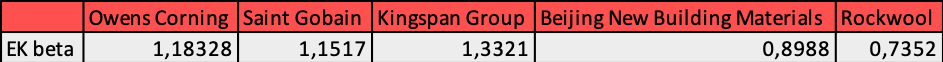
\includegraphics[width=\linewidth]{tabeller/ekbeta.png}
  \caption{Sammenlignbare egenkapitalbeta}
  \label{tbl:ekbeta}
\end{table}

Vi har benyttet den representative hovedindeksen til hvert enkelt selskap basert på hvor det er notert. Ut i fra tabellen kan man lese at alle selskaper har en positiv korrelasjon med hovedindeksen, men Rockwool er det selskapet som fluktuerer minst i forhold til markedet.

\indent \newline
Etter at egenkapitalbetaen er beregnet må denne regnes om til eiendelsbeta. Dette utføres ved å vekte gjeldsandelen med gjeldsbetaen, og egenkapitalsandelen med egenkapitalbetaen. 

\[\beta_E = \frac{G}{(G + E)} * \beta_G + (1 - \frac{G}{(G + E)}) * \beta_{EK}\]
\textit{hvor:
\begin{itemize}
    \item[] $\beta_E$ = sammenlignbare selskapers eiendelsbeta
    \item[] $G$ = Markedsverdi rentebærende gjeld
    \item[] $\beta_G$ = Gjeldsbeta
    \item[] $E$ = Markedsverdi egenkapital
\end{itemize}
}

\begin{table}[H]
  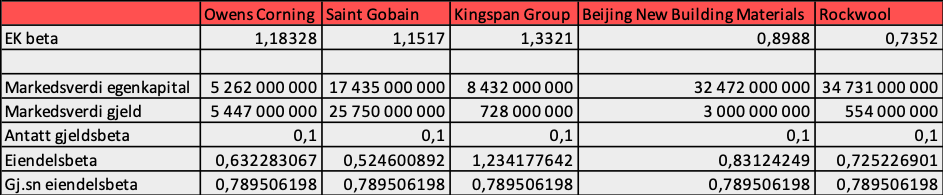
\includegraphics[width=\linewidth]{tabeller/eiendelsbetasammenlignbare.png}
  \caption{Sammenlignbare eiendelsbeta}
  \label{tbl:eiendelsbetasammenlignbare}
\end{table}

Fra dette finner vi gjennomsnittlig eiendelsbeta for de sammenlignbare selskapene til å være 0,7895. For å finne relevant beta for Rockwool må dette estimatet regnes om til egenkapitalbeta. Formelen for egenkapitalbeta er: 

\[\beta_{EK} = \frac{(\beta_E - \beta_G) * G}{(1 - G)}\]
\textit{hvor:
\begin{itemize}
    \item[] $\beta_{EK}$ = Egenkapitalbeta
    \item[] $\beta_E$ = Likeveid gjennomsnitt av sammenlignbare selskapers eiendelsbeta
    \item[] $\beta_G$ = Gjeldsbeta
    \item[] $G$ = Markedsverdibasert gjeldsandel
\end{itemize}
}

\[\beta_{EK} = \frac{(0,7895 - 0,1) * (\frac{554.000.000}{34.731.000.000})}{1 - (\frac{554.000.000}{34.731.000.000})}\]
\[\beta_{EK} = 0,7719\]

Begge metodene resulterer i relativt like betaer. Vi velger å legge den første beregningen, som kun målte ROCKWOOL International korrelasjon, til grunn for videre analyse.

\subsection{Estimering av gjeldskostnad}
Ved investeringsbeslutninger vil ikke selve finansieringen av prosjektet, enten det er egenkapitalfinansiert eller gjeldsfinansiert, spille noen rolle for prosjektets gjeldsandel. Logikken bak dette ligger i at det er selskapet som står ansvarlig for gjelden, långiver vil derfor ikke bistå med midler til et prosjekt uten å ta hensyn til selskapet. 

\indent \newline
Investeringen finansieres gjennom støtte fra Enova og interne midler fra konsernet. Prosjektet krever derfor ikke opptak av ny gjeld. For å beregne relevant gjeldskostnad til avkastningskravet tar vi derfor utgangspunkt i regnskapstall fra ROCKWOOL International. Vi beregner gjeldskostnaden ved å se på rentekostnaden dividert med inngående rentebærende gjeld summert med rentebærende låneopptak for det relevante regnskapsåret. Vi finner det hensiktsmessig å bruke fjorårets (2018 tall) regnskapstall \cite{proffdk}. 

\[\frac{12.000.000}{236.000.000} = 5,08\%\]

\subsection{Blumes justeringsmodell}
Analyser gjennomført av Marshall Blume viser at selskapers betaverdier tenderer å bevege seg mot 1, og at selskaper med betaverdier nære 1 er mer stabile enn de som er lenger unna. Blume mente derfor at det er hensiktsmessig å justere betaen med følgende modell:

\[\beta_{justert} = \beta_{raw} * P +1,0 *(1-P)\]
\textit{hvor:
\begin{itemize}
    \item[] $P$ = estimeringsfeilen (0,67)
    \item[] $1,0$ = markedets betaverdi
\end{itemize}
}
Nyere forskning støtter opp under resonnementet til Blume for prosjekter med lang tidshorisont. I vår analyse som strekker seg over 20 år velger vi derfor å  benytte oss av \textit{mean reversion} \cite{forelesningsnotater}.

\[\beta_{justert} = 0,735266 * 0,6667 + 1,0 * (1 - 0,6667) = 0,8235\]

\subsection{Beregning av egenkapitalens avkastningskrav}
\[k_E = rf * (1-s) + \beta_{EK} * [E(r_m)-rf * (1-s)] \]
\[k_E =0,0171*(1-0,22)+0,8235*[0,05-0,0171*(1-0,22)]\]
\[k_E =0,04353\]
\begin{center}Se seksjon \ref{sec:ekavkast} for mer informasjon.\end{center}

\subsection{Beregning av totalkapitalens avkastningskrav}
\[k_T = k_E * \frac{E}{E + G} + k_G * (1-s) * \frac{G}{E + G}\]
\[k_T = 0,04353*0,8235+0,0508*(1-0,22)*0,2188\]
\[k_T = 4,35\%\]
\begin{center}Se seksjon \ref{sec:totavkast} for mer informasjon.\end{center}

\subsection{Valutarisiko} 
Et relevant tema som følger av investeringer over landegrenser er valuta- og landsrisiko. Ettersom ROCKWOOL International er et multinasjonalt selskap med fabrikker over hele verden vil eierne være eksponert mot slik risiko. Som følge av landsrisiko foreligger faktorer som politikk, legale, finansielle med mer. I en netto nåverdianalyse inkluderes denne risikoen ved enten å justere de forventede kontantstrømmene, eller justere avkastningskravet. Vi har valgt å inkludere valutaeksponeringen eierne og kreditorer står overfor gjennom å justere avkastningskravet. Ved behandlingen av landsrisiko som er knyttet til de politiske og legale aspektet anser vi risikoen i prosjektet som lik selskapsrisikoen. I henhold til Damodarans utredelse av landsrisiko er dette en riktig forutsetning \cite{adamodar}.

\indent \newline
Historiske tall viser til høy volatilitet mellom den norske og danske kronen. I tider der den norske kronen styrker seg mot den danske vil kontantstrømmen til konsernet bli lavere, og motsatt.

\begin{figure}[H]
  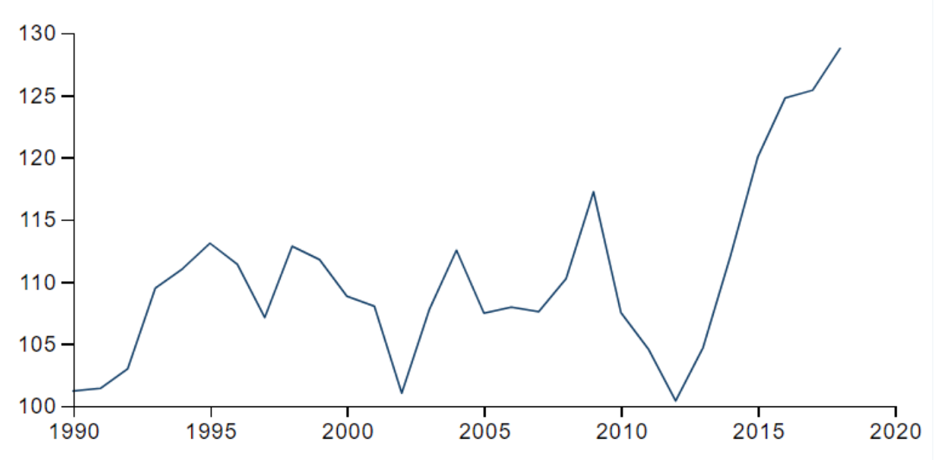
\includegraphics[width=\linewidth]{bilder/valutahistorikk.png}
  \caption{Valutakurssvingninger}
  \label{fig:valutahistorikk}
\end{figure}

Tabellen viser den årlige svingningen i valutakursen mellom den danske og norske kronene gjennom de siste 40 årene. Disse svingningene gjør eierne til ROCKWOOL International utsatt for økt risiko knyttet til kontantstrømsutbetalingen.  

\indent \newline
Vi legger derfor til grunn en valutarisiko på 1,4\%.

\subsection{Business risk}
Investeringen vil ta i bruk produksjonsteknologi som ikke er testet ut i like stor skala tidligere, og medfører derfor økt risiko i den operasjonelle driften. Innkjøringsperioden er estimert til tre måneder og innebærer full produksjonsstopp. Ved at selskapet selv må utvikle nødvendige løsninger for å tilpasse teknologien til produksjonsanlegget, er det en fare for at innkjøringsperioden kan ta lenger tid enn forventet. Det ligger med andre ord usikkerhet i å oppnå effektiv utnyttelse av ovnen sett opp mot volumene resten av produksjonsanlegget er tilpasset til. I tillegg vil det oppstå hyppigere nedetid i produksjonen i forbindelse med skifting av lining inne i ovnen. Det er også rimelig å anta forekomst av uforutsette produksjonsstopp, spesielt de første årene grunnet manglende erfaring med teknologien.

\indent \newline
Selskapet opererer med et standard påslag på 2\% på totalkapitalkravet ved investeringer som innehar normal business risk. Da dette er et pilotprosjekt for konsernet, legger vi til grunn en business risk på 3\%.

\subsection{Relevant avkastningskrav (WACC)}
\[Relevant_{WACC} = WACC + valutarisiko + business risk\]
\[Relevant_{WACC} = 4,35\% + 1,4\% + 3\% = 8,75\%\]

\subsection{Internrentemetoden}
Internrenten forklarer den faktiske avkastningen på prosjektet. Ved å diskontere kontantstrømmene med internrenten vil netto nåverdi dermed bli null. Dette gir en tolkning om at alle avkastningskrav høyere enn internrenten vil gi negativ netto nåverdi. Ettersom internrenten kun er et mål på lønnsomheten vil vi kun benytte oss av metoden som et supplement til den tradisjonelle netto nåverdimetoden.

\subsection{Konsistensbetingelser}
En forutsetning for at netto nåverdianalysen skal forme et realistisk bilde av lønnsomheten er at benyttede data er konsistente. Dette innebærer at alle tallstørrelser som er relevante i forhold til hverandre behandles med like utgangspunkt. For denne type lønnsomhetsanalyser er det i all hovedsak rammebetingelsene for kontantstrømmen og avkastningskravet som skal være like. Det kan eksempelvis ikke inkluderes skatt i kontantstrømmen dersom man ikke også inkluderer det i avkastningskravet. Slike feil vil forme et urealistisk bilde av analysen. I denne oppgaven sammenligner vi to alternativer gjennom en differansekontantstrøm. I likhet med forutsetningen om å behandle kontantstrøm og avkastningskrav konsistent må også kontantstrømmene behandles konsistent i forhold til hverandre. Det innebærer blant annet at forutsetninger om fremtidig markedsutvikling må være lik i begge alternativene. Konsistensbetingelsene vi legger til grunn er som følger:

\begin{itemize}
\item Nominelle tall
\item Utregning av kontantstrøm og avkastningskrav vil bli beregnet etter fratrukket skatt ettersom skattereduksjonen aldri er lik i teller og nevner
\item Lik periodelengde
\item Totalkapitalmetoden
\end{itemize}

\section{Markedseffisiens}
I netto nåverdiberegninger bør resultatet alltid drøftes i lys av effisiensbegrepet. I et effisient marked vil prisene fullt ut reflektere tilgjengelig informasjon. Det betyr at det ikke skal være mulig å oppnå en ekstraordinær avkastning på investert kapital. Dette danner grunnlaget for at man alltid må kunne forklare hvorfor prosjektet klarer å oppnå denne meravkastningen. Bakgrunnen for ekstraordinær avkastning kan da foreligge dersom et marked er ineffisient. Dette innebærer at ikke all tilgjengelig informasjon er priset inn i markedet. Hvis dette er tilfellet vil det foreligge en arbitrasjemulighet, det vil si at investor kan oppnå ekstra avkastning uten å påta seg økt risiko. Dette vil likevel ikke vare evig ettersom arbitrasjører vil benytte seg av muligheten for meravkastning helt til likevekt er oppnådd. En annen forklaring ligger i at netto nåverdiberegningen er gal. Dette kan fremkomme av en overvurdering i kontantstrømmene, undervurdering av avkastningskravet eller begge deler.




